\chapter{Dataset and evaluation metrics}
\label{chap:dataset}
\section{UOT100 Dataset}
Underwater Object Tracking (UOT100) is a benchmark dataset designed to facilitate the development and evaluation of object tracking algorithms specifically tailored for underwater environments \cite{kezebou2019underwater,panetta2021comprehensive}. Unlike traditional tracking datasets that focus on open-air scenarios, UOT100 addresses the unique challenges posed by underwater visual data, including light attenuation, refraction, scattering, and color loss. These distortions significantly impact object visibility and tracking accuracy, making the dataset a crucial resource for advancing research in underwater object tracking.

\begin{figure}[ht]
    \centering
    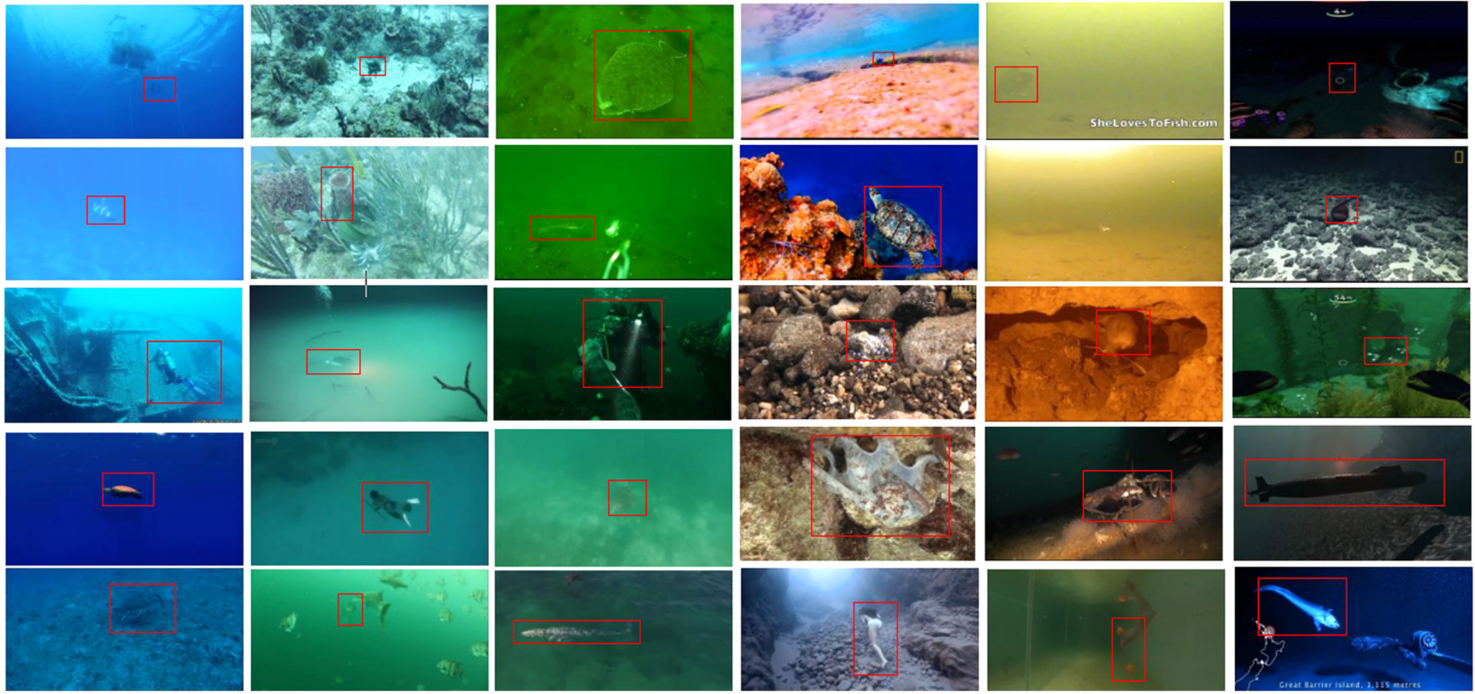
\includegraphics[width=0.8\textwidth]{images/uot100.png}
    \caption{Sample frames from the UOT100 dataset, showcasing various underwater conditions and distortions.}
    \label{fig:uot100_samples}
\end{figure}

The UOT100 dataset consists of 104 video sequences with over 74,000 manually annotated frames. These sequences encompass a diverse range of underwater conditions, including both natural and artificial environments. The dataset includes various types of distortions, such as low contrast, motion blur, occlusions, and fluctuating illumination, which are common in real-world underwater applications.

Each video sequence in the dataset is accompanied by:
\begin{itemize}
    \item An MP4 video file capturing the object of interest.
    \item A ground truth annotation file containing the precise bounding box coordinates for the tracked object.
    \item A description file outlining the distortion types present in the video.
    \item An image sequence folder that stores individual frames for more granular analysis.
\end{itemize}

The dataset is publicly available for research purposes and serves as a standard benchmark for comparing the performance of state-of-the-art tracking algorithms in underwater conditions. It provides a foundation for assessing the robustness of correlation filter-based and deep learning-based tracking methods when applied to challenging aquatic environments



\section{Evaluation Metrics}

To objectively assess the performance of object tracking algorithms on the UOT100 dataset, we employ standard evaluation metrics commonly used in the tracking community. These metrics include \textbf{Average Overlap (AO)}, \textbf{Success Rate (SR)}, \textbf{Success Curve}, and \textbf{Frames Per Second (FPS)}, all of which provide a comprehensive evaluation of both accuracy and computational efficiency. The selected metrics align with those utilized in the GOT10k benchmark, ensuring comparability with state-of-the-art trackers \cite{wu2013online}.

\subsection{Average Overlap (AO)}
Average Overlap (AO) measures the mean Intersection over Union (IoU) between the predicted bounding box and the ground truth bounding box over the entire dataset. This metric provides an overall indication of how well a tracker maintains accurate localization of the target throughout the sequence. AO is defined as:

\begin{equation}
AO = \frac{1}{N} \sum_{i=1}^{N} IoU_i
\end{equation}

where $N$ is the total number of frames in the dataset, and $IoU_i$ represents the Intersection over Union in frame $i$.

\subsection{Success Rate (SR)}
Success Rate (SR) evaluates the proportion of frames in which the IoU between the predicted and ground truth bounding boxes exceeds a predefined threshold. Two widely used thresholds are 0.5 (SR${0.5}$) and 0.75 (SR${0.75}$), which indicate the fraction of frames where the overlap meets or surpasses these respective values. A higher SR value signifies a more reliable tracker, particularly in challenging underwater environments.

\subsection{Success Curve}
The Success Curve visualizes the Success Rate over a range of IoU thresholds, offering a more detailed perspective on a tracker’s performance across different levels of accuracy requirements. The Area Under Curve (AUC) of the Success Curve is often reported as a single scalar value to summarize the overall tracking effectiveness \cite{wu2013online}.

\subsection{Frames Per Second (FPS)}
Frames Per Second (FPS) measures the computational efficiency of a tracking algorithm, reflecting its capability for real-time processing. A higher FPS value indicates lower computational overhead, making the tracker more suitable for real-time underwater applications such as autonomous underwater vehicles (AUVs) and marine surveillance.

By employing these metrics, the UOT100 benchmark provides a standardized and rigorous evaluation framework for comparing object tracking algorithms in underwater environments.

\endinput